\documentclass[11pt]{article}
\usepackage[margin=18mm,headheight=22pt]{geometry}
\usepackage{amsmath}
\usepackage{fontspec}
\usepackage{unicode-math}
\setmainfont{NewCM10}[Extension=.otf,UprightFont=*-Book,BoldFont=*-Bold,ItalicFont=*-BookItalic,BoldItalicFont=*-BoldItalic]
\setsansfont{NewCMSans10}[Extension=.otf,UprightFont=*-Book,BoldFont=*-Bold,ItalicFont=*-BookOblique,BoldItalicFont=*-BoldOblique]
\setmathfont{NewCMMath-Book.otf}
\usepackage{xcolor}
\definecolor{FAUblue}{HTML}{04316A}
\definecolor{Paperblue}{HTML}{EEF2F7}
\definecolor{EEIgold}{HTML}{CC9C42}
\usepackage{etoolbox,enumitem,booktabs,tabularx,array,needspace,microtype}
\usepackage[most]{tcolorbox}
\usepackage{titlesec,fancyhdr}
\usepackage[hidelinks]{hyperref}
\usepackage{draftwatermark}
\SetWatermarkText{Made by Thanate Amornjiraporn (Focus)}
\SetWatermarkColor{black!7}\SetWatermarkFontSize{30pt}\SetWatermarkAngle{45}
\setlength{\parindent}{0pt}
\setlength{\parskip}{5pt}
\setlist{itemsep=2pt,topsep=3pt,leftmargin=1.6em,beginpenalty=10000,endpenalty=10000}
\raggedbottom
\clubpenalty=10000 \widowpenalty=10000 \displaywidowpenalty=10000 \interlinepenalty=10000
\setcounter{secnumdepth}{0}
\setcounter{tocdepth}{1}
\pagestyle{fancy}\fancyhf{}
\fancyhead[L]{\small\sffamily\color{FAUblue} From Fundamentals to AI Apocalypse · MEI · Exercise Sheet 2}
\fancyhead[R]{\small\sffamily Exercise 2: Worked solutions}
\fancyfoot[C]{\small\thepage}
\titleformat{\section}{\Large\bfseries\sffamily\color{FAUblue}}{}{0pt}{}
\titleformat{\subsection}{\large\bfseries\sffamily\color{FAUblue}}{}{0pt}{}
\titlespacing*{\section}{0pt}{16pt}{6pt}
\preto\section{\Needspace{8\baselineskip}}
\preto\subsection{\Needspace{6\baselineskip}}
\newtcolorbox{equationcard}[1]{colback=Paperblue,colframe=Paperblue,boxrule=0pt,arc=0pt,left=10pt,right=10pt,top=6pt,bottom=6pt,title={#1},fonttitle=\small\bfseries\sffamily,coltitle=FAUblue,before skip=8pt,after skip=8pt}
\newtcolorbox{workedbox}[1]{colback=white,colframe=EEIgold,boxrule=0pt,leftrule=3pt,arc=0pt,left=10pt,top=4pt,bottom=4pt,title={#1},fonttitle=\small\bfseries\sffamily,coltitle=FAUblue,attach title to upper={\par},before skip=8pt,after skip=8pt}
\newtcolorbox{recallbox}[1]{colback=white,colframe=FAUblue,boxrule=0pt,leftrule=3pt,arc=0pt,left=10pt,top=4pt,bottom=4pt,title={#1},fonttitle=\small\bfseries\sffamily,coltitle=FAUblue,attach title to upper={\par},before skip=8pt,after skip=8pt}
\usepackage{environ}
\newsavebox\measurebox
% Typeset the section once invisibly to measure it; start a new page if it will not fit in what is left.
\makeatletter
\newif\ifkeep@measuring
\NewEnviron{keepsection}{%
  \ifkeep@measuring \BODY \else
    \edef\keep@sec{\the\value{section}}\edef\keep@sub{\the\value{subsection}}%
    \setbox\measurebox\vbox{\hsize\linewidth\keep@measuringtrue\def\Needspace##1{}\BODY}%
    \setcounter{section}{\keep@sec}\setcounter{subsection}{\keep@sub}%
    \dimen2=\ht\measurebox \advance\dimen2\dp\measurebox
    \dimen@=\textheight
    \ifdim\pagegoal<\maxdimen
      \dimen@=\pagegoal \advance\dimen@-\pagetotal
      \ifdim\dimen2>\dimen@ \clearpage \dimen@=\textheight \fi
    \fi
    % if it fits, nothing inside may force an early break
    \ifdim\dimen2>\dimen@ \BODY \else \begingroup\def\Needspace##1{}\BODY\endgroup \fi
  \fi}
\makeatother
\newtcolorbox{notebox}{colback=Paperblue,colframe=Paperblue,boxrule=0pt,arc=0pt,left=8pt,right=8pt,top=4pt,bottom=4pt,before skip=6pt,after skip=6pt}
\newtcolorbox{plainbox}{colback=white,colframe=FAUblue,boxrule=0pt,leftrule=3pt,arc=0pt,left=10pt,right=8pt,top=4pt,bottom=4pt,before skip=6pt,after skip=8pt}
\usetikzlibrary{arrows.meta}
\title{\sffamily\bfseries\color{FAUblue}Exercise 2: Worked solutions}
\author{Mathematics for Engineers I \ensuremath{\cdot} Module 62765 \ensuremath{\cdot} Exercise Sheet 2\\[2pt]\small From Fundamentals to AI Apocalypse · personal study guide}
\date{}
\begin{document}
\maketitle
\begingroup\footnotesize\setlength{\parskip}{0pt}\tableofcontents\endgroup
\clearpage

\begin{keepsection}
\Needspace{9\baselineskip}
\section{Exercise 2.1: Absolute values and inequalities}

\Needspace{6\baselineskip}
Absolute value is distance from zero. Splitting at sign changes turns these expressions into ordinary inequalities on intervals.

\textbf{Connected topic:} Absolute values and inequalities (§2.3) explain the distance interpretation and safe case splitting.

\begin{keepsection}
\Needspace{6\baselineskip}
\subsection{1a(i): Sketch \textit{x}\textsuperscript{2} \ensuremath{-} 2|\textit{y}| \ensuremath{>} 1}

\Needspace{3\baselineskip}
Try first: isolate |\textit{y}|, then check where the resulting upper bound is non-negative.

\nopagebreak[4]{\small\itshape Answers: see “Exercise 2.1: Absolute values and inequalities” under Answers at the end.}
\end{keepsection}

\begin{keepsection}
\Needspace{6\baselineskip}
\subsection{1a(ii): Sketch |\textit{x}| + |\textit{y}| = 2}

\Needspace{3\baselineskip}
Try first: split the plane into quadrants and find where the boundary meets each axis.

\nopagebreak[4]{\small\itshape Answers: see “Exercise 2.1: Absolute values and inequalities” under Answers at the end.}
\end{keepsection}

\begin{keepsection}
\Needspace{6\baselineskip}
\subsection{1b(i): Solve |\textit{x} + 1| \ensuremath{-} |\textit{x} \ensuremath{-} 1| = 1}

\Needspace{3\baselineskip}
Try first: split at \ensuremath{-}1 and 1, where the expressions inside the absolute values change sign.

\nopagebreak[4]{\small\itshape Answers: see “Exercise 2.1: Absolute values and inequalities” under Answers at the end.}
\end{keepsection}

\begin{keepsection}
\Needspace{7\baselineskip}
\subsection{1b(ii): Solve \ensuremath{\sqrt{{x}\, -\, 12}} \ensuremath{<} \textit{x} \ensuremath{-} 2}

\Needspace{4\baselineskip}
Try first: write the square-root domain and make sure both sides are non-negative before squaring.

\nopagebreak[4]{\small\itshape Answers: see “Exercise 2.1: Absolute values and inequalities” under Answers at the end.}
\end{keepsection}
\end{keepsection}

\begin{keepsection}
\Needspace{9\baselineskip}
\section{Exercise 2.2: Supremum and infimum}

\Needspace{6\baselineskip}
A supremum is a least upper bound; it need not be a member of the set. A maximum must belong to the set, and the same distinction applies to infimum and minimum.

\textbf{Connected topic:} Real numbers, completeness, supremum and infimum (§2.2) give the bound definitions and the ε-characterisation used here.

\begin{keepsection}
\Needspace{7\baselineskip}
\subsection{2a(i): Find the bounds and extrema of \textit{M}\textsubscript{1} = (0, 1]}

\Needspace{4\baselineskip}
Try first: identify the numbers approached at both ends and check which endpoints the interval includes.

\nopagebreak[4]{\small\itshape Answers: see “Exercise 2.2: Supremum and infimum” under Answers at the end.}
\end{keepsection}

\begin{keepsection}
\Needspace{6\baselineskip}
\subsection{2a(ii): Find the bounds and extrema of \textit{M}\textsubscript{2} = \{{\small\ensuremath{\dfrac{1}{{n}}}} : \textit{n} \ensuremath{\in} \ensuremath{\mathbb{N}}\}}

\Needspace{3\baselineskip}
Try first: list the first few values and determine their limit as \textit{n} grows.

\nopagebreak[4]{\small\itshape Answers: see “Exercise 2.2: Supremum and infimum” under Answers at the end.}
\end{keepsection}

\begin{keepsection}
\Needspace{7\baselineskip}
\subsection{2a(iii): Find the bounds and extrema of \textit{M}\textsubscript{3} = \{ (\ensuremath{-}1)\textsuperscript{\textit{n}}(1 + {\small\ensuremath{\dfrac{1}{{n}}}}) : \textit{n} \ensuremath{\in} \ensuremath{\mathbb{N}} \}}

\Needspace{4\baselineskip}
Try first: separate even \textit{n} from odd \textit{n}; their signs differ, so each subsequence controls a different extreme.

\nopagebreak[4]{\small\itshape Answers: see “Exercise 2.2: Supremum and infimum” under Answers at the end.}
\end{keepsection}

\begin{keepsection}
\Needspace{7\baselineskip}
\subsection{2b: Show that \textit{M} = \{\textit{x} \ensuremath{\in} \ensuremath{\mathbb{Q}} : \textit{x}\textsuperscript{2} \ensuremath{<} 2\} has infinitely many rational upper bounds but no rational supremum}

\Needspace{4\baselineskip}
Try first: show that every rational greater than \ensuremath{\sqrt{2}} is an upper bound, then ask whether such a bound can be the least rational one.

\nopagebreak[4]{\small\itshape Answers: see “Exercise 2.2: Supremum and infimum” under Answers at the end.}
\end{keepsection}
\end{keepsection}

\begin{keepsection}
\Needspace{9\baselineskip}
\section{Exercise 2.3: Sums, products, binomial coefficients}

\Needspace{6\baselineskip}
Use index changes to expose patterns, cancellation to simplify sums, and combinations to count pairs or selections.

\textbf{Connected topic:} Sums, products and binomial coefficients (§2.4) define the notation, geometric sums and counting rules used below.

\begin{keepsection}
\Needspace{6\baselineskip}
\subsection{3a: Write the odd square numbers from 121 to 2401 as a sum}

\Needspace{3\baselineskip}
Try first: represent the odd bases as a sequence with step 2, starting at 11 and ending at 49.

\nopagebreak[4]{\small\itshape Answers: see “Exercise 2.3: Sums, products, binomial coefficients” under Answers at the end.}
\end{keepsection}

\begin{keepsection}
\Needspace{7\baselineskip}
\subsection{3b(i): Simplify the difference of two sums}

\Needspace{4\baselineskip}
Try first: shift the first index so both sums contain the same powers of \textit{x}, then compare coefficients.

\nopagebreak[4]{\small\itshape Answers: see “Exercise 2.3: Sums, products, binomial coefficients” under Answers at the end.}
\end{keepsection}

\begin{keepsection}
\Needspace{7\baselineskip}
\subsection{3b(ii): Compute the nested sum and product}

\Needspace{4\baselineskip}
Try first: evaluate the inner product for each \textit{m}; look for a zero factor before multiplying numbers.

\nopagebreak[4]{\small\itshape Answers: see “Exercise 2.3: Sums, products, binomial coefficients” under Answers at the end.}
\end{keepsection}

\begin{keepsection}
\Needspace{6\baselineskip}
\subsection{3b(iii): Simplify the sum of C(\textit{n}, \textit{k}) over \textit{k}}

\Needspace{3\baselineskip}
Try first: use the binomial theorem with both entries equal to 1.

\nopagebreak[4]{\small\itshape Answers: see “Exercise 2.3: Sums, products, binomial coefficients” under Answers at the end.}
\end{keepsection}

\begin{keepsection}
\Needspace{6\baselineskip}
\subsection{3c: Find the number of guests from 66 clinks}

\Needspace{3\baselineskip}
Try first: one clink corresponds to one unordered pair of distinct guests.

\nopagebreak[4]{\small\itshape Answers: see “Exercise 2.3: Sums, products, binomial coefficients” under Answers at the end.}
\end{keepsection}

\begin{keepsection}
\Needspace{7\baselineskip}
\subsection{3d: Birthday probability for 27 students}

\Needspace{4\baselineskip}
Try first: calculate the complement event that every birthday is different, then subtract from 1.

\nopagebreak[4]{\small\itshape Answers: see “Exercise 2.3: Sums, products, binomial coefficients” under Answers at the end.}
\end{keepsection}
\end{keepsection}

\begin{keepsection}
\Needspace{10\baselineskip}
\section{Exercise 2.4: Order axioms}

\Needspace{7\baselineskip}
Each result follows from the field and order axioms, not from assuming familiar arithmetic laws. Use uniqueness of inverses, distributivity, trichotomy, and compatibility of order with addition and positive multiplication.

\textbf{Connected topic:} Real numbers as an ordered field (§2.2) lists the axioms from which each identity and inequality is derived.

\begin{keepsection}
\Needspace{6\baselineskip}
\subsection{4i: Prove \textit{a} \ensuremath{\cdot} 0 = 0}

\Needspace{3\baselineskip}
Try first: write 0 as 0 + 0 and use distributivity, then cancel a term from both sides.

\nopagebreak[4]{\small\itshape Answers: see “Exercise 2.4: Order axioms” under Answers at the end.}
\end{keepsection}

\begin{keepsection}
\Needspace{7\baselineskip}
\subsection{4ii: Prove \ensuremath{-}\textit{a} = (\ensuremath{-}1)\ensuremath{\cdot}\textit{a}}

\Needspace{4\baselineskip}
Try first: show that (\ensuremath{-}1)\ensuremath{\cdot}\textit{a} added to \textit{a} equals zero, then use uniqueness of the additive inverse.

\nopagebreak[4]{\small\itshape Answers: see “Exercise 2.4: Order axioms” under Answers at the end.}
\end{keepsection}

\begin{keepsection}
\Needspace{7\baselineskip}
\subsection{4iii: Prove (\ensuremath{-}\textit{a})\ensuremath{\cdot}(\ensuremath{-}\textit{b}) = \textit{a}\ensuremath{\cdot}\textit{b}}

\Needspace{4\baselineskip}
Try first: replace each negative by multiplication by \ensuremath{-}1; establish (\ensuremath{-}1)(\ensuremath{-}1) = 1 from part ii).

\nopagebreak[4]{\small\itshape Answers: see “Exercise 2.4: Order axioms” under Answers at the end.}
\end{keepsection}

\begin{keepsection}
\Needspace{7\baselineskip}
\subsection{4iv: Prove \textit{a}\textit{b} = 0 \ensuremath{\Rightarrow} \textit{a} = 0 or \textit{b} = 0}

\Needspace{4\baselineskip}
Try first: assume \textit{a} \ensuremath{\neq} 0 so its multiplicative inverse exists, then multiply the equation by that inverse.

\nopagebreak[4]{\small\itshape Answers: see “Exercise 2.4: Order axioms” under Answers at the end.}
\end{keepsection}

\begin{keepsection}
\Needspace{6\baselineskip}
\subsection{4v: Prove 1 \ensuremath{>} 0}

\Needspace{3\baselineskip}
Try first: use trichotomy and rule out 1 = 0 and 1 \ensuremath{<} 0.

\nopagebreak[4]{\small\itshape Answers: see “Exercise 2.4: Order axioms” under Answers at the end.}
\end{keepsection}

\begin{keepsection}
\Needspace{6\baselineskip}
\subsection{4vi: Prove \textit{a}\textsuperscript{2} \ensuremath{>} 0 for \textit{a} \ensuremath{\neq} 0}

\Needspace{3\baselineskip}
Try first: split into \textit{a} \ensuremath{>} 0 and \textit{a} \ensuremath{<} 0, and express the second square using \ensuremath{-}\textit{a}.

\nopagebreak[4]{\small\itshape Answers: see “Exercise 2.4: Order axioms” under Answers at the end.}
\end{keepsection}

\begin{keepsection}
\Needspace{6\baselineskip}
\subsection{4vii: Show \textit{a} \ensuremath{<} \textit{b} and \textit{c} \ensuremath{<} 0 imply \textit{a}\textit{c} \ensuremath{>} \textit{b}\textit{c}}

\Needspace{3\baselineskip}
Try first: translate \textit{a} \ensuremath{<} \textit{b} into a positive difference, and identify the sign of \textit{c}(\textit{b} \ensuremath{-} \textit{a}).

\nopagebreak[4]{\small\itshape Answers: see “Exercise 2.4: Order axioms” under Answers at the end.}
\end{keepsection}
\end{keepsection}

\begin{keepsection}
\Needspace{9\baselineskip}
\section{Self-Study 2.5: Absolute values and inequalities}

\Needspace{6\baselineskip}
The first condition describes a diamond in the plane; the one-variable inequalities are handled by splitting intervals and checking domains before squaring.

\textbf{Connected topic:} Absolute values and inequalities (§2.3) connect distance regions with interval solutions.

\begin{keepsection}
\Needspace{7\baselineskip}
\subsection{5a: Sketch |\textit{x}| + |\textit{y} \ensuremath{-} 2| \ensuremath{<} 5}

\Needspace{4\baselineskip}
Try first: interpret each term as a distance from a coordinate, then locate the four axis-parallel intercepts.

\nopagebreak[4]{\small\itshape Answers: see “Self-Study 2.5: Absolute values and inequalities” under Answers at the end.}
\end{keepsection}

\begin{keepsection}
\Needspace{6\baselineskip}
\subsection{5b(i): Solve |\textit{x} + 3| + |\textit{x} \ensuremath{-} 3| \ensuremath{>} 8}

\Needspace{3\baselineskip}
Try first: inside [\ensuremath{-}3,3] the two distances add to a constant; outside it they grow with |\textit{x}|.

\nopagebreak[4]{\small\itshape Answers: see “Self-Study 2.5: Absolute values and inequalities” under Answers at the end.}
\end{keepsection}

\begin{keepsection}
\Needspace{6\baselineskip}
\subsection{5b(ii): Solve \ensuremath{\sqrt{({x}\, -\, 4)({x}\, -\, 1)}} \ensuremath{\leq} 2 \ensuremath{-} \textit{x}}

\Needspace{3\baselineskip}
Try first: require a non-negative radicand and a non-negative right side before squaring.

\nopagebreak[4]{\small\itshape Answers: see “Self-Study 2.5: Absolute values and inequalities” under Answers at the end.}
\end{keepsection}
\end{keepsection}

\begin{keepsection}
\Needspace{9\baselineskip}
\section{Self-Study 2.6: Sets, products and complements}

\Needspace{6\baselineskip}
Use ordered-pair membership for products and remember that every complement depends on its declared universe.

\textbf{Connected topic:} Set inclusion, Cartesian products and complements (§1.2) define the membership tests used below.

\begin{keepsection}
\Needspace{6\baselineskip}
\subsection{6a: Prove \textit{A} \ensuremath{\times} \textit{B} \ensuremath{\subset} \textit{C} \ensuremath{\times} \textit{D} when \textit{A} \ensuremath{\subset} \textit{C} and \textit{B} \ensuremath{\subset} \textit{D}}

\Needspace{3\baselineskip}
Try first: take an arbitrary ordered pair from \textit{A} \ensuremath{\times} \textit{B} and track each coordinate separately.

\nopagebreak[4]{\small\itshape Answers: see “Self-Study 2.6: Sets, products and complements” under Answers at the end.}
\end{keepsection}

\begin{keepsection}
\Needspace{7\baselineskip}
\subsection{6b: Is the converse true?}

\Needspace{4\baselineskip}
Try first: ask what happens when one Cartesian-product factor is empty, so the product contains no pairs.

\nopagebreak[4]{\small\itshape Answers: see “Self-Study 2.6: Sets, products and complements” under Answers at the end.}
\end{keepsection}

\begin{keepsection}
\Needspace{7\baselineskip}
\subsection{6c: Compute the complements and difference for \textit{A} = [1,3), \textit{B} = (2,5] in \textit{X} = \ensuremath{\mathbb{R}}}

\Needspace{4\baselineskip}
Try first: mark each endpoint, then form the union and intersection before taking their complements relative to \ensuremath{\mathbb{R}}.

\nopagebreak[4]{\small\itshape Answers: see “Self-Study 2.6: Sets, products and complements” under Answers at the end.}
\end{keepsection}

\begin{keepsection}
\Needspace{7\baselineskip}
\subsection{6d: Find the complement of [1,3] \ensuremath{\times} [1,2] in \ensuremath{\mathbb{R}}\textsuperscript{2}}

\Needspace{4\baselineskip}
Try first: a point is outside the rectangle if at least one coordinate lies outside its own closed interval.

\nopagebreak[4]{\small\itshape Answers: see “Self-Study 2.6: Sets, products and complements” under Answers at the end.}
\end{keepsection}
\end{keepsection}

\begin{keepsection}
\Needspace{9\baselineskip}
\section{Self-Study 2.7: Sums, products, binomial coefficients}

\Needspace{6\baselineskip}
Match each term to an index, telescope products before expanding them, and use combinations when order does not matter.

\textbf{Connected topic:} Sums, products and binomial coefficients (§2.4) supply the geometric, telescoping and counting identities.

\begin{keepsection}
\Needspace{7\baselineskip}
\subsection{7a: Write 10\textsuperscript{2} \ensuremath{-} {\small\ensuremath{\dfrac{1}{9^{2}}}} + 8\textsuperscript{2} \ensuremath{-} {\small\ensuremath{\dfrac{1}{7^{2}}}} + … + 2\textsuperscript{2} \ensuremath{-} {\small\ensuremath{\dfrac{1}{1^{2}}}} as a sum}

\Needspace{4\baselineskip}
Try first: choose an index that makes the positive bases descend by 2 from 10 and the denominators descend from 9.

\nopagebreak[4]{\small\itshape Answers: see “Self-Study 2.7: Sums, products, binomial coefficients” under Answers at the end.}
\end{keepsection}

\begin{keepsection}
\Needspace{6\baselineskip}
\subsection{7b(i): Simplify the difference of geometric sums}

\Needspace{3\baselineskip}
Try first: write out the powers in both sums and look for the unmatched term.

\nopagebreak[4]{\small\itshape Answers: see “Self-Study 2.7: Sums, products, binomial coefficients” under Answers at the end.}
\end{keepsection}

\begin{keepsection}
\Needspace{7\baselineskip}
\subsection{7b(ii): Simplify the product}

\Needspace{4\baselineskip}
Try first: factor the numerator \textit{j}(\textit{j}+1) \ensuremath{-} 2 and separate the product into two telescoping ratios.

\nopagebreak[4]{\small\itshape Answers: see “Self-Study 2.7: Sums, products, binomial coefficients” under Answers at the end.}
\end{keepsection}

\begin{keepsection}
\Needspace{6\baselineskip}
\subsection{7b(iii): Simplify the alternating binomial sum}

\Needspace{3\baselineskip}
Try first: expand (1 + \textit{x})\textsuperscript{\textit{n}} and substitute \textit{x} = \ensuremath{-}1.

\nopagebreak[4]{\small\itshape Answers: see “Self-Study 2.7: Sums, products, binomial coefficients” under Answers at the end.}
\end{keepsection}

\begin{keepsection}
\Needspace{7\baselineskip}
\subsection{7c: Pick six marbles with at most two striped marbles}

\Needspace{4\baselineskip}
Try first: remember there are only four white marbles, so any six-marble selection must include at least two striped ones.

\nopagebreak[4]{\small\itshape Answers: see “Self-Study 2.7: Sums, products, binomial coefficients” under Answers at the end.}
\end{keepsection}

\begin{keepsection}
\Needspace{7\baselineskip}
\subsection{7d: Find the members from 272 spoken riddles}

\Needspace{4\baselineskip}
Try first: distinguish a greeting spoken from one unordered pair. Each member speaks once to each of the other members.

\nopagebreak[4]{\small\itshape Answers: see “Self-Study 2.7: Sums, products, binomial coefficients” under Answers at the end.}
\end{keepsection}
\end{keepsection}


\clearpage
\section{Answers}
\begin{keepsection}\subsection{Exercise 2.1: Absolute values and inequalities}

\begin{workedbox}{1a(i) \ensuremath{\cdot} Two unbounded curved bands}
\Needspace{14\baselineskip}
\begin{enumerate}
\item Move the absolute-value term to the right: 2|\textit{y}| \ensuremath{<} \textit{x}\textsuperscript{2} \ensuremath{-} 1. Since the left side is non-negative, solutions require \textit{x}\textsuperscript{2} \ensuremath{-} 1 \ensuremath{>} 0, so |\textit{x}| \ensuremath{>} 1.
\item \Needspace{4\baselineskip}
For those \textit{x}, divide by 2 and remove the absolute value as a two-sided bound:

\begin{equation*}-\dfrac{{x}^{2}\, -\, 1}{2}\, <\, {y}\, <\, \dfrac{{x}^{2}\, -\, 1}{2},\, \text{for}\, {x}\, <\, -1\, \text{or}\, {x}\, >\, 1\end{equation*}
\item The solution is the interior between the curves \textit{y} = \ensuremath{\pm}{\small\ensuremath{\dfrac{{x}^{2}\, -\, 1}{2}}} on the two outer sides |\textit{x}| \ensuremath{>} 1. The curves and the vertical cutoffs \textit{x} = \ensuremath{\pm}1 are excluded. At |\textit{x}| = 1 the only possible \textit{y} would be 0, but the original inequality is strict and fails there.
\item \Needspace{9\baselineskip}
\textbf{Check:} at \textit{x} = 2, the condition is |\textit{y}| \ensuremath{<} {\small\ensuremath{\dfrac{3}{2}}}; at \textit{x} = 0 it has no solution.

\Needspace{14\baselineskip}
\begin{center}
\begin{minipage}[t]{0.950\linewidth}\centering
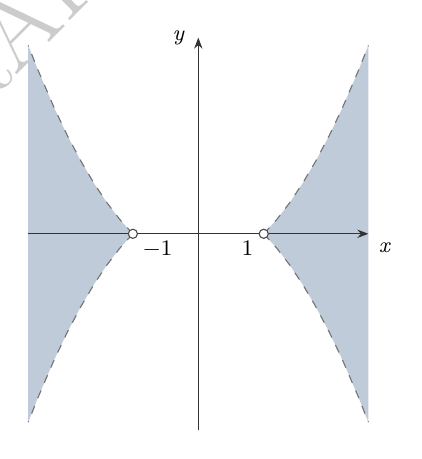
\begin{tikzpicture}[line join=round]
\fill[FAUblue!25] (3.423,-2.924) -- (3.589,-2.742) -- (3.755,-2.526) -- (3.921,-2.276) -- (4.087,-1.994) -- (4.254,-1.678) -- (4.420,-1.329) -- (4.627,-0.847) -- (4.752,-0.532) -- (4.752,-5.317) -- (4.627,-5.001) -- (4.420,-4.519) -- (4.254,-4.170) -- (4.087,-3.855) -- (3.921,-3.572) -- (3.755,-3.323) -- (3.589,-3.107) -- cycle;
\fill[FAUblue!25] (1.761,-2.924) -- (1.595,-2.742) -- (1.429,-2.526) -- (1.263,-2.276) -- (1.097,-1.994) -- (0.930,-1.678) -- (0.764,-1.329) -- (0.557,-0.847) -- (0.432,-0.532) -- (0.432,-5.317) -- (0.557,-5.001) -- (0.764,-4.519) -- (0.930,-4.170) -- (1.097,-3.855) -- (1.263,-3.572) -- (1.429,-3.323) -- (1.595,-3.107) -- cycle;
\draw[-{Stealth[length=4pt]},black!80] (0.432,-2.924) -- (4.752,-2.924);
\node[anchor=west,fill=white,fill opacity=0.85,text opacity=1,inner sep=1pt,font=\footnotesize] at (4.842,-3.104) {\textit{x}};
\draw[-{Stealth[length=4pt]},black!80] (2.592,-5.417) -- (2.592,-0.432);
\node[anchor=east,fill=white,fill opacity=0.85,text opacity=1,inner sep=1pt,font=\footnotesize] at (2.466,-0.432) {\textit{y}};
\draw[black!55,dashed] (3.423,-2.924) -- (3.589,-2.742) -- (3.755,-2.526) -- (3.921,-2.276) -- (4.087,-1.994) -- (4.254,-1.678) -- (4.420,-1.329) -- (4.627,-0.847) -- (4.752,-0.532);
\draw[black!55,dashed] (3.423,-2.924) -- (3.589,-3.107) -- (3.755,-3.323) -- (3.921,-3.572) -- (4.087,-3.855) -- (4.254,-4.170) -- (4.420,-4.519) -- (4.627,-5.001) -- (4.752,-5.317);
\draw[black!55,dashed] (1.761,-2.924) -- (1.595,-2.742) -- (1.429,-2.526) -- (1.263,-2.276) -- (1.097,-1.994) -- (0.930,-1.678) -- (0.764,-1.329) -- (0.557,-0.847) -- (0.432,-0.532);
\draw[black!55,dashed] (1.761,-2.924) -- (1.595,-3.107) -- (1.429,-3.323) -- (1.263,-3.572) -- (1.097,-3.855) -- (0.930,-4.170) -- (0.764,-4.519) -- (0.557,-5.001) -- (0.432,-5.317);
\draw[draw=black!70,fill=white] (1.761,-2.924) circle (0.058);
\draw[draw=black!70,fill=white] (3.423,-2.924) circle (0.058);
\node[anchor=west,fill=white,fill opacity=0.85,text opacity=1,inner sep=1pt,font=\footnotesize] at (1.851,-3.104) {\ensuremath{-}1};
\node[anchor=east,fill=white,fill opacity=0.85,text opacity=1,inner sep=1pt,font=\footnotesize] at (3.333,-3.104) {1};
\end{tikzpicture}\par\smallskip{\small\raggedright \textbf{Boundary of \textit{x}\textsuperscript{2} \ensuremath{-} 2|\textit{y}| \ensuremath{>} 1.} The shaded bands are the solution set; the dashed curves and the open points at (\ensuremath{\pm}1, 0) are excluded, and the bands lie between the curves where |\textit{x}| \ensuremath{>} 1. The gap for \ensuremath{-}1 \ensuremath{<} \textit{x} \ensuremath{<} 1 has no solutions.\par}\end{minipage}
\end{center}
\end{enumerate}
\end{workedbox}

\end{keepsection}
\begin{keepsection}\subsection{Exercise 2.1: Absolute values and inequalities}

\begin{workedbox}{1a(ii) \ensuremath{\cdot} A diamond boundary}
\Needspace{11\baselineskip}
\begin{enumerate}
\item On each quadrant, replace absolute values by the corresponding signed coordinates. For example, when \textit{x} \ensuremath{\geq} 0 and \textit{y} \ensuremath{\geq} 0, the equation is \textit{x} + \textit{y} = 2.
\item Setting one coordinate to zero gives the four vertices (2, 0), (0, 2), (\ensuremath{-}2, 0), and (0, \ensuremath{-}2). Between consecutive vertices the equation is linear.
\item Join those points with straight segments and include the whole boundary, because equality is required. The enclosed diamond itself is not the requested set.
\item \Needspace{8\baselineskip}
\textbf{Check:} (1, 1) lies on it; (0, 0) and (2, 2) do not.

\Needspace{14\baselineskip}
\begin{center}
\begin{minipage}[t]{0.950\linewidth}\centering
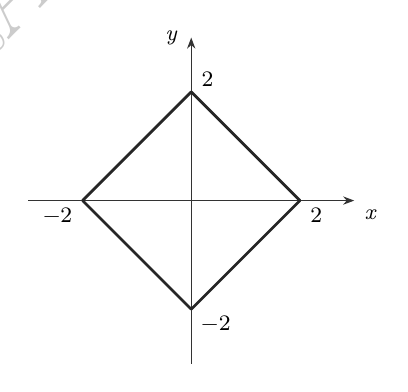
\begin{tikzpicture}[line join=round]
\draw[-{Stealth[length=4pt]},black!80] (0.432,-2.502) -- (4.572,-2.502);
\node[anchor=west,fill=white,fill opacity=0.85,text opacity=1,inner sep=1pt,font=\footnotesize] at (4.662,-2.682) {\textit{x}};
\draw[-{Stealth[length=4pt]},black!80] (2.502,-4.572) -- (2.502,-0.432);
\node[anchor=east,fill=white,fill opacity=0.85,text opacity=1,inner sep=1pt,font=\footnotesize] at (2.376,-0.432) {\textit{y}};
\draw[black!85,line width=1pt] (1.122,-2.502) -- (2.502,-1.122) -- (3.882,-2.502) -- (2.502,-3.882) -- (1.122,-2.502);
\node[anchor=west,fill=white,fill opacity=0.85,text opacity=1,inner sep=1pt,font=\footnotesize] at (2.592,-0.960) {2};
\node[anchor=west,fill=white,fill opacity=0.85,text opacity=1,inner sep=1pt,font=\footnotesize] at (3.972,-2.682) {2};
\node[anchor=west,fill=white,fill opacity=0.85,text opacity=1,inner sep=1pt,font=\footnotesize] at (2.592,-4.062) {\ensuremath{-}2};
\node[anchor=east,fill=white,fill opacity=0.85,text opacity=1,inner sep=1pt,font=\footnotesize] at (1.032,-2.682) {\ensuremath{-}2};
\end{tikzpicture}\par\smallskip{\small\raggedright \textbf{|\textit{x}| + |\textit{y}| = 2.} The four straight sides join the intercepts. The equality keeps only this outline, not the region inside it.\par}\end{minipage}
\end{center}
\end{enumerate}
\end{workedbox}

\end{keepsection}
\begin{keepsection}\subsection{Exercise 2.1: Absolute values and inequalities}

\begin{workedbox}{1b(i) \ensuremath{\cdot} Solve by intervals}
\Needspace{10\baselineskip}
\begin{enumerate}
\item If \textit{x} \ensuremath{\leq} \ensuremath{-}1, both distances simplify to \ensuremath{-}(\textit{x}+1) and \ensuremath{-}(\textit{x}\ensuremath{-}1); their difference is \ensuremath{-}2, so there is no solution there.
\item If \ensuremath{-}1 \ensuremath{\leq} \textit{x} \ensuremath{\leq} 1, the expression is (\textit{x}+1) \ensuremath{-} (1\ensuremath{-}\textit{x}) = 2\textit{x}. Setting 2\textit{x} = 1 gives \textit{x} = {\small\ensuremath{\dfrac{1}{2}}}, which lies in this interval.
\item If \textit{x} \ensuremath{\geq} 1, the expression is (\textit{x}+1) \ensuremath{-} (\textit{x}\ensuremath{-}1) = 2, not 1.
\item \textbf{Answer:} \{{\small\ensuremath{\dfrac{1}{2}}}\}. The interval check is essential: each simplified equation is valid only in its own case.
\end{enumerate}
\end{workedbox}

\end{keepsection}
\begin{keepsection}\subsection{Exercise 2.1: Absolute values and inequalities}

\begin{workedbox}{1b(ii) \ensuremath{\cdot} Domain first, then square}
\Needspace{9\baselineskip}
\begin{enumerate}
\item The radicand requires \textit{x} \ensuremath{-} 12 \ensuremath{\geq} 0, so \textit{x} \ensuremath{\geq} 12. On this domain, \textit{x} \ensuremath{-} 2 \ensuremath{\geq} 10, so both sides are non-negative and squaring preserves the inequality.
\item \Needspace{4\baselineskip}
Square and simplify:

\begin{equation*}{x}\, -\, 12\, <\, ({x}\, -\, 2)^{2}\, \Leftrightarrow \, 0\, <\, {x}^{2}\, -\, 5{x}\, +\, 16\end{equation*}
\item The quadratic is always positive: its discriminant is 25 \ensuremath{-} 64 = \ensuremath{-}39 \ensuremath{<} 0 and its leading coefficient is positive. Thus every \textit{x} in the domain works.
\item \textbf{Answer:} [12, \ensuremath{\infty}). For instance, \textit{x} = 12 gives 0 \ensuremath{<} 10, confirming the boundary is included.
\end{enumerate}
\end{workedbox}

\end{keepsection}
\begin{keepsection}\subsection{Exercise 2.2: Supremum and infimum}

\begin{workedbox}{2a \ensuremath{\cdot} The half-open interval}
\Needspace{7\baselineskip}
\begin{enumerate}
\item Every member is at most 1, and 1 belongs to \textit{M}\textsubscript{1}. Therefore sup \textit{M}\textsubscript{1} = max \textit{M}\textsubscript{1} = 1.
\item Every member is positive, so 0 is a lower bound. Values can be chosen arbitrarily close to 0 from above, so no larger number is a lower bound. Thus inf \textit{M}\textsubscript{1} = 0.
\item Because 0 is not in the interval, \textit{M}\textsubscript{1} has no minimum. \textbf{Summary:} sup = max = 1; inf = 0; no minimum.
\end{enumerate}
\end{workedbox}

\end{keepsection}
\begin{keepsection}\subsection{Exercise 2.2: Supremum and infimum}

\begin{workedbox}{2a \ensuremath{\cdot} A decreasing sequence of reciprocals}
\Needspace{8\baselineskip}
\begin{enumerate}
\item Here \ensuremath{\mathbb{N}} = \{1, 2, …\}, as defined in the MEI notes. The first term is 1, and {\small\ensuremath{\dfrac{1}{{n}}}} \ensuremath{\leq} 1 for every positive \textit{n}, so sup \textit{M}\textsubscript{2} = max \textit{M}\textsubscript{2} = 1.
\item All terms are positive. Given any ε \ensuremath{>} 0, choose a natural \textit{n} \ensuremath{>} {\small\ensuremath{\dfrac{1}{ε}}}; then {\small\ensuremath{\dfrac{1}{{n}}}} \ensuremath{<} ε. Hence no positive number is a lower bound, and inf \textit{M}\textsubscript{2} = 0.
\item Zero is not one of the terms, so there is no minimum. \textbf{Summary:} sup = max = 1; inf = 0; no minimum.
\end{enumerate}
\end{workedbox}

\end{keepsection}
\begin{keepsection}\subsection{Exercise 2.2: Supremum and infimum}

\begin{workedbox}{2a \ensuremath{\cdot} Separate positive and negative terms}
\Needspace{7\baselineskip}
\begin{enumerate}
\item For odd \textit{n}, the terms are negative: \ensuremath{-}(1 + {\small\ensuremath{\dfrac{1}{{n}}}}). Their smallest value occurs at the smallest odd \textit{n}, \textit{n} = 1, giving \ensuremath{-}2. All later negative terms are greater than \ensuremath{-}2.
\item For even \textit{n}, terms are positive: 1 + {\small\ensuremath{\dfrac{1}{{n}}}}. Their largest value occurs at the smallest even \textit{n}, \textit{n} = 2, giving {\small\ensuremath{\dfrac{3}{2}}}. All later positive terms are smaller.
\item \textbf{Summary:} inf \textit{M}\textsubscript{3} = min \textit{M}\textsubscript{3} = \ensuremath{-}2; sup \textit{M}\textsubscript{3} = max \textit{M}\textsubscript{3} = {\small\ensuremath{\dfrac{3}{2}}}. Both bounds are attained.
\end{enumerate}
\end{workedbox}

\end{keepsection}
\begin{keepsection}\subsection{Exercise 2.2: Supremum and infimum}

\begin{workedbox}{2b \ensuremath{\cdot} The least upper bound is irrational}
\Needspace{13\baselineskip}
\begin{enumerate}
\item \textit{M} is non-empty (1 \ensuremath{\in} \textit{M}), and every \textit{x} \ensuremath{\in} \textit{M} satisfies \textit{x} \ensuremath{<} \ensuremath{\sqrt{2}}. Each rational \textit{q} \ensuremath{>} \ensuremath{\sqrt{2}} is therefore an upper bound. There are infinitely many: for example, choose \textit{q} = 2 + {\small\ensuremath{\dfrac{1}{{n}}}} for each positive integer \textit{n}; all exceed \ensuremath{\sqrt{2}} and give distinct rationals.
\item Suppose a rational \textit{S} were sup\textsubscript{\ensuremath{\mathbb{Q}}} \textit{M}. All members of \textit{M} lie below \ensuremath{\sqrt{2}}, and rationals in \textit{M} approach it from below because \ensuremath{\mathbb{Q}} is dense in \ensuremath{\mathbb{R}}. Thus \ensuremath{\sqrt{2}} is the real least upper bound.
\item By the given ε-characterisation, a supremum \textit{S} must be an upper bound, so \textit{S} \ensuremath{\geq} \ensuremath{\sqrt{2}}. For every ε \ensuremath{>} 0, there is \textit{x} \ensuremath{\in} \textit{M} with \textit{x} \ensuremath{>} \textit{S} \ensuremath{-} ε, while every \textit{x} \ensuremath{\in} \textit{M} is below \ensuremath{\sqrt{2}}; hence \textit{S} \ensuremath{-} ε \ensuremath{<} \ensuremath{\sqrt{2}} for every ε, forcing \textit{S} \ensuremath{\leq} \ensuremath{\sqrt{2}}. Therefore \textit{S} = \ensuremath{\sqrt{2}}. But that is irrational, contradicting \textit{S} \ensuremath{\in} \ensuremath{\mathbb{Q}}.
\item \textbf{Conclusion:} \textit{M} has infinitely many upper bounds in \ensuremath{\mathbb{Q}} but no supremum in \ensuremath{\mathbb{Q}}. In \ensuremath{\mathbb{R}} its supremum is \ensuremath{\sqrt{2}}.
\end{enumerate}
\end{workedbox}

\end{keepsection}
\begin{keepsection}\subsection{Exercise 2.3: Sums, products, binomial coefficients}

\begin{workedbox}{3a \ensuremath{\cdot} Index the odd bases}
\Needspace{7\baselineskip}
\begin{enumerate}
\item The odd integers in the stated range are 11, 13, …, 49. Starting with \textit{k} = 0, the kth base is 11 + 2\textit{k}. It reaches 49 when \textit{k} = 19.
\item \Needspace{4\baselineskip}
Therefore the requested sum is:

\begin{equation*}\sum_{{k}=0}^{19} \, (11\, +\, 2{k})^{2}\end{equation*}
\item \textbf{Check:} the first term is 11\textsuperscript{2} = 121 and the last is (11 + 38)\textsuperscript{2} = 49\textsuperscript{2} = 2401; there are 20 odd squares.
\end{enumerate}
\end{workedbox}

\end{keepsection}
\begin{keepsection}\subsection{Exercise 2.3: Sums, products, binomial coefficients}

\begin{workedbox}{3b(i) \ensuremath{\cdot} Coefficient cancellation}
\Needspace{10\baselineskip}
\begin{enumerate}
\item Re-index the first sum with \textit{j} = \textit{k} + 1. The bracket becomes $\sum_{{j}=1}^{10} $ \textit{j}\textit{x}\textsuperscript{\textit{j}} \ensuremath{-} $\sum_{{j}=0}^{10} $ (\textit{j} + 1)\textit{x}\textsuperscript{\textit{j}}.
\item The constant term is \ensuremath{-}1. For each power \textit{x}\textsuperscript{\textit{j}}, 1 \ensuremath{\leq} \textit{j} \ensuremath{\leq} 10, the coefficient is \textit{j} \ensuremath{-} (\textit{j} + 1) = \ensuremath{-}1. Thus the bracket is \ensuremath{-}(1 + \textit{x} + … + \textit{x}\textsuperscript{10}).
\item \Needspace{4\baselineskip}
Multiply by (1 \ensuremath{-} \textit{x}) and use the finite geometric-sum identity:

\begin{equation*}-(1\, -\, {x})(1\, +\, {x}\, +\, …\, +\, {x}^{10})\, =\, -(1\, -\, {x}^{11})\, =\, {x}^{11}\, -\, 1\end{equation*}
\item \textbf{Answer:} \textit{x}\textsuperscript{11} \ensuremath{-} 1, valid for every real \textit{x}, including \textit{x} = 1 because the polynomial identity has no division by 1 \ensuremath{-} \textit{x}.
\end{enumerate}
\end{workedbox}

\end{keepsection}
\begin{keepsection}\subsection{Exercise 2.3: Sums, products, binomial coefficients}

\begin{workedbox}{3b(ii) \ensuremath{\cdot} A zero term removes one product}
\Needspace{6\baselineskip}
\begin{enumerate}
\item At \textit{m} = 1, the product includes \textit{k} = 1, whose factor is 1\textsuperscript{2} \ensuremath{-} 1 = 0. That whole inner product is 0.
\item \Needspace{4\baselineskip}
At \textit{m} = 2, the product has \textit{k} = 2 and \textit{k} = 3:

\begin{equation*}(2^{2}\, -\, 1)(3^{2}\, -\, 1)\, =\, 3\, \cdot \, 8\, =\, 24\end{equation*}
\item Add the two outer terms: 0 + 24 = \textbf{24}.
\end{enumerate}
\end{workedbox}

\end{keepsection}
\begin{keepsection}\subsection{Exercise 2.3: Sums, products, binomial coefficients}

\begin{workedbox}{3b(iii) \ensuremath{\cdot} Count all subsets}
\Needspace{6\baselineskip}
\begin{enumerate}
\item \Needspace{4\baselineskip}
Expand (1 + 1)\textsuperscript{\textit{n}} by the binomial theorem:

\begin{equation*}(1\, +\, 1)^{{n}}\, =\, \sum_{{k}=0}^{{n}} \, \mathrm{C}({n},\, {k})\, \cdot \, 1^{{n}-{k}}\, \cdot \, 1^{{k}}\end{equation*}
\item Every power of 1 equals 1, so the requested sum equals 2\textsuperscript{\textit{n}}. This also counts all subsets of an \textit{n}-element set.
\item \textbf{Answer:} 2\textsuperscript{\textit{n}}.
\end{enumerate}
\end{workedbox}

\end{keepsection}
\begin{keepsection}\subsection{Exercise 2.3: Sums, products, binomial coefficients}

\begin{workedbox}{3c \ensuremath{\cdot} Count unordered pairs}
\Needspace{7\baselineskip}
\begin{enumerate}
\item With \textit{g} guests, every pair clinks once, so the number of clinks is C(\textit{g},2) = {\small\ensuremath{\dfrac{{g}({g}\, -\, 1)}{2}}}.
\item \Needspace{4\baselineskip}
Set the count to 66 and solve:

\begin{equation*}\dfrac{{g}({g}\, -\, 1)}{2}\, =\, 66\, \Leftrightarrow \, {g}^{2}\, -\, {g}\, -\, 132\, =\, 0\, \Leftrightarrow \, ({g}\, -\, 12)({g}\, +\, 11)\, =\, 0\end{equation*}
\item The roots are 12 and \ensuremath{-}11; only a positive guest count is possible. \textbf{There are 12 guests.}
\item \textbf{Check:} 12\ensuremath{\cdot}{\small\ensuremath{\dfrac{11}{2}}} = 66 distinct pairs.
\end{enumerate}
\end{workedbox}

\end{keepsection}
\begin{keepsection}\subsection{Exercise 2.3: Sums, products, binomial coefficients}

\begin{workedbox}{3d \ensuremath{\cdot} Use the complement probability}
\Needspace{10\baselineskip}
\begin{enumerate}
\item Assume independent, equally likely birthdays on 365 days, as specified. The first student can have any birthday; for no match, the next has 364 choices, then 363, continuing down to 339 choices for the 27th student.
\item \Needspace{4\baselineskip}
There are 365\textsuperscript{27} equally likely birthday assignments overall. Hence:

\Needspace{4\baselineskip}
\begin{equation*}\mathrm{P}(\text{all}\, \text{birthdays}\, \text{different})\, =\, \dfrac{365\, \cdot \, 364\, \cdot \, …\, \cdot \, 339}{365^{27}}\end{equation*}

\begin{equation*}\mathrm{P}(\text{at}\, \text{least}\, \text{one}\, \text{shared}\, \text{birthday})\, =\, 1\, -\, \dfrac{365\, \cdot \, 364\, \cdot \, …\, \cdot \, 339}{365^{27}}\, \approx \, 0.6269\end{equation*}
\item \textbf{Answer:} about 62.7\%. This is the probability of at least one matching pair, not the expected number of matching pairs.
\end{enumerate}
\end{workedbox}

\end{keepsection}
\begin{keepsection}\subsection{Exercise 2.4: Order axioms}

\begin{workedbox}{4i \ensuremath{\cdot} Distributivity and cancellation}
\Needspace{7\baselineskip}
\begin{enumerate}
\item Since 0 = 0 + 0, distributivity gives \textit{a}\ensuremath{\cdot}0 = \textit{a}(0 + 0) = \textit{a}\ensuremath{\cdot}0 + \textit{a}\ensuremath{\cdot}0.
\item Add the additive inverse of \textit{a}\ensuremath{\cdot}0 to both sides. The left becomes 0 and the right becomes \textit{a}\ensuremath{\cdot}0, so \textbf{\textit{a}\ensuremath{\cdot}0 = 0}.
\item This argument works for every \textit{a} and uses only the additive identity, distributivity and additive inverses.
\end{enumerate}
\end{workedbox}

\end{keepsection}
\begin{keepsection}\subsection{Exercise 2.4: Order axioms}

\begin{workedbox}{4ii \ensuremath{\cdot} Identify the additive inverse}
\Needspace{5\baselineskip}
\begin{enumerate}
\item Distributivity gives (\ensuremath{-}1)\ensuremath{\cdot}\textit{a} + \textit{a} = ((\ensuremath{-}1) + 1)\ensuremath{\cdot}\textit{a}.
\item (\ensuremath{-}1) + 1 = 0, and part i) gives 0\ensuremath{\cdot}\textit{a} = 0. Therefore (\ensuremath{-}1)\ensuremath{\cdot}\textit{a} + \textit{a} = 0.
\item An additive inverse is unique, so \textbf{(\ensuremath{-}1)\ensuremath{\cdot}\textit{a} = \ensuremath{-}\textit{a}}.
\end{enumerate}
\end{workedbox}

\end{keepsection}
\begin{keepsection}\subsection{Exercise 2.4: Order axioms}

\begin{workedbox}{4iii \ensuremath{\cdot} Two negative factors}
\Needspace{7\baselineskip}
\begin{enumerate}
\item Part ii) gives \ensuremath{-}\textit{a} = (\ensuremath{-}1)\textit{a} and \ensuremath{-}\textit{b} = (\ensuremath{-}1)\textit{b}. Associativity and commutativity of multiplication then give (\ensuremath{-}\textit{a})(\ensuremath{-}\textit{b}) = ((\ensuremath{-}1)(\ensuremath{-}1))(\textit{a}\textit{b}).
\item Apply part ii) to the element \ensuremath{-}1: \ensuremath{-}(\ensuremath{-}1) = (\ensuremath{-}1)(\ensuremath{-}1). The additive inverse of \ensuremath{-}1 is 1, so this product equals 1.
\item Thus (\ensuremath{-}\textit{a})(\ensuremath{-}\textit{b}) = 1\ensuremath{\cdot}\textit{a}\textit{b} = \textbf{\textit{a}\textit{b}}.
\end{enumerate}
\end{workedbox}

\end{keepsection}
\begin{keepsection}\subsection{Exercise 2.4: Order axioms}

\begin{workedbox}{4iv \ensuremath{\cdot} Use the inverse of a non-zero factor}
\Needspace{9\baselineskip}
\begin{enumerate}
\item Suppose \textit{a}\textit{b} = 0. If \textit{a} = 0, the conclusion already holds.
\item \Needspace{4\baselineskip}
Otherwise \textit{a} \ensuremath{\neq} 0, so \textit{a}\textsuperscript{\ensuremath{-}1} exists in the field. Multiply \textit{a}\textit{b} = 0 by \textit{a}\textsuperscript{\ensuremath{-}1}:

\begin{equation*}{a}^{-1}({a}{b})\, =\, {a}^{-1}\, \cdot \, 0\end{equation*}
\item Associativity and the zero-product result from i) reduce this to \textit{b} = 0. In either case, \textbf{\textit{a} = 0 or \textit{b} = 0}.
\item The existence of inverses for non-zero elements is the crucial field property; it need not hold in an arbitrary ring.
\end{enumerate}
\end{workedbox}

\end{keepsection}
\begin{keepsection}\subsection{Exercise 2.4: Order axioms}

\begin{workedbox}{4v \ensuremath{\cdot} Exclude the other order cases}
\Needspace{8\baselineskip}
\begin{enumerate}
\item In a field, 1 \ensuremath{\neq} 0. Trichotomy therefore leaves either 1 \ensuremath{>} 0 or 1 \ensuremath{<} 0.
\item Assume for contradiction that 1 \ensuremath{<} 0. Add \ensuremath{-}1 to both sides: 0 \ensuremath{<} \ensuremath{-}1.
\item The product of two positive elements is positive, so (\ensuremath{-}1)(\ensuremath{-}1) \ensuremath{>} 0. Part iii), or the identity established in its proof, says (\ensuremath{-}1)(\ensuremath{-}1) = 1. Thus 1 \ensuremath{>} 0, contradicting 1 \ensuremath{<} 0.
\item The negative case is impossible. Therefore \textbf{1 \ensuremath{>} 0}.
\end{enumerate}
\end{workedbox}

\end{keepsection}
\begin{keepsection}\subsection{Exercise 2.4: Order axioms}

\begin{workedbox}{4vi \ensuremath{\cdot} A non-zero square is positive}
\Needspace{7\baselineskip}
\begin{enumerate}
\item By trichotomy, \textit{a} \ensuremath{\neq} 0 means either \textit{a} \ensuremath{>} 0 or \textit{a} \ensuremath{<} 0.
\item If \textit{a} \ensuremath{>} 0, the product of positive elements gives \textit{a}\ensuremath{\cdot}\textit{a} \ensuremath{>} 0.
\item If \textit{a} \ensuremath{<} 0, then \ensuremath{-}\textit{a} \ensuremath{>} 0. Its square is positive, and part iii) gives (\ensuremath{-}\textit{a})(\ensuremath{-}\textit{a}) = \textit{a}\ensuremath{\cdot}\textit{a}.
\item Both cases establish \textbf{\textit{a}\textsuperscript{2} \ensuremath{>} 0}.
\end{enumerate}
\end{workedbox}

\end{keepsection}
\begin{keepsection}\subsection{Exercise 2.4: Order axioms}

\begin{workedbox}{4vii \ensuremath{\cdot} Multiplication by a negative reverses order}
\Needspace{8\baselineskip}
\begin{enumerate}
\item Add \ensuremath{-}\textit{a} to the inequality \textit{a} \ensuremath{<} \textit{b}. Compatibility of order with addition gives 0 \ensuremath{<} \textit{b} \ensuremath{-} \textit{a}.
\item Because \ensuremath{-}\textit{c} \ensuremath{>} 0 and \textit{b} \ensuremath{-} \textit{a} \ensuremath{>} 0, the product (\ensuremath{-}\textit{c})(\textit{b} \ensuremath{-} \textit{a}) is positive. The identity (\ensuremath{-}\textit{c})(\textit{b} \ensuremath{-} \textit{a}) = \ensuremath{-}(\textit{c}(\textit{b} \ensuremath{-} \textit{a})) follows from distributivity and additive inverses, so \textit{c}(\textit{b} \ensuremath{-} \textit{a}) \ensuremath{<} 0.
\item Expand: \textit{c}(\textit{b} \ensuremath{-} \textit{a}) = \textit{c}\textit{b} \ensuremath{-} \textit{c}\textit{a} \ensuremath{<} 0. Add \textit{c}\textit{a} to both sides to obtain \textit{c}\textit{b} \ensuremath{<} \textit{c}\textit{a}.
\item Commutativity gives \textbf{\textit{a}\textit{c} \ensuremath{>} \textit{b}\textit{c}}. The direction reverses because \textit{c} is negative.
\end{enumerate}
\end{workedbox}

\end{keepsection}
\begin{keepsection}\subsection{Self-Study 2.5: Absolute values and inequalities}

\begin{workedbox}{5a \ensuremath{\cdot} Interior of a translated diamond}
\Needspace{9\baselineskip}
\begin{enumerate}
\item |\textit{x}| is horizontal distance from \textit{x} = 0; |\textit{y} \ensuremath{-} 2| is vertical distance from \textit{y} = 2. Their sum is the Manhattan distance from (0, 2).
\item Set one distance to zero to find the vertices: \textit{x} = \ensuremath{\pm}5 when \textit{y} = 2; and \textit{y} \ensuremath{-} 2 = \ensuremath{\pm}5 when \textit{x} = 0, giving \textit{y} = 7 and \textit{y} = \ensuremath{-}3.
\item \Needspace{9\baselineskip}
The strict inequality keeps the interior of the diamond with vertices (\ensuremath{-}5,2), (5,2), (0,7), and (0,\ensuremath{-}3). The boundary is excluded.

\Needspace{14\baselineskip}
\begin{center}
\begin{minipage}[t]{0.950\linewidth}\centering
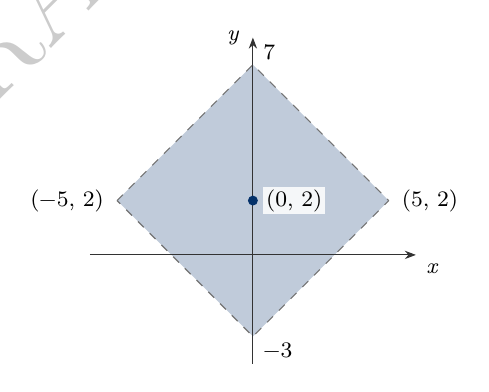
\begin{tikzpicture}[line join=round]
\fill[FAUblue!25] (0.777,-2.502) -- (2.502,-0.777) -- (4.227,-2.502) -- (2.502,-4.227) -- cycle;
\draw[-{Stealth[length=4pt]},black!80] (0.432,-3.192) -- (4.572,-3.192);
\node[anchor=west,fill=white,fill opacity=0.85,text opacity=1,inner sep=1pt,font=\footnotesize] at (4.662,-3.372) {\textit{x}};
\draw[-{Stealth[length=4pt]},black!80] (2.502,-4.572) -- (2.502,-0.432);
\node[anchor=east,fill=white,fill opacity=0.85,text opacity=1,inner sep=1pt,font=\footnotesize] at (2.376,-0.432) {\textit{y}};
\draw[black!55,dashed] (0.777,-2.502) -- (2.502,-0.777) -- (4.227,-2.502) -- (2.502,-4.227) -- (0.777,-2.502);
\fill[FAUblue] (2.502,-2.502) circle (0.063);
\node[anchor=west,fill=white,fill opacity=0.85,text opacity=1,inner sep=1pt,font=\footnotesize] at (2.628,-2.502) {(0, 2)};
\node[anchor=west,fill=white,fill opacity=0.85,text opacity=1,inner sep=1pt,font=\footnotesize] at (4.353,-2.502) {(5, 2)};
\node[anchor=east,fill=white,fill opacity=0.85,text opacity=1,inner sep=1pt,font=\footnotesize] at (0.651,-2.502) {(\ensuremath{-}5, 2)};
\node[anchor=west,fill=white,fill opacity=0.85,text opacity=1,inner sep=1pt,font=\footnotesize] at (2.592,-0.615) {7};
\node[anchor=west,fill=white,fill opacity=0.85,text opacity=1,inner sep=1pt,font=\footnotesize] at (2.592,-4.407) {\ensuremath{-}3};
\end{tikzpicture}\par\smallskip{\small\raggedright \textbf{|\textit{x}| + |\textit{y} \ensuremath{-} 2| \ensuremath{<} 5.} The shaded interior, centred at (0, 2), is the solution set; the dashed boundary is excluded.\par}\end{minipage}
\end{center}
\end{enumerate}
\end{workedbox}

\end{keepsection}
\begin{keepsection}\subsection{Self-Study 2.5: Absolute values and inequalities}

\begin{workedbox}{5b(i) \ensuremath{\cdot} Sum of distances from two points}
\Needspace{9\baselineskip}
\begin{enumerate}
\item For \ensuremath{-}3 \ensuremath{\leq} \textit{x} \ensuremath{\leq} 3, |\textit{x}+3| = \textit{x}+3 and |\textit{x}\ensuremath{-}3| = 3\ensuremath{-}\textit{x}. Their sum is 6, which is not greater than 8.
\item For \textit{x} \ensuremath{>} 3, both terms are positive expressions, so the sum is (\textit{x}+3)+(\textit{x}\ensuremath{-}3)=2\textit{x}. The inequality gives \textit{x} \ensuremath{>} 4.
\item For \textit{x} \ensuremath{<} \ensuremath{-}3, both absolute values reverse sign and the sum is \ensuremath{-}2\textit{x}. Then \ensuremath{-}2\textit{x} \ensuremath{>} 8 gives \textit{x} \ensuremath{<} \ensuremath{-}4.
\item \textbf{Answer:} (\ensuremath{-}\ensuremath{\infty}, \ensuremath{-}4) \ensuremath{\cup} (4, \ensuremath{\infty}). The endpoints are excluded because the original inequality is strict.
\end{enumerate}
\end{workedbox}

\end{keepsection}
\begin{keepsection}\subsection{Self-Study 2.5: Absolute values and inequalities}

\begin{workedbox}{5b(ii) \ensuremath{\cdot} Combine domain restrictions, then square}
\Needspace{10\baselineskip}
\begin{enumerate}
\item The radicand is non-negative when \textit{x} \ensuremath{\leq} 1 or \textit{x} \ensuremath{\geq} 4. Since a square root is non-negative, the right side 2 \ensuremath{-} \textit{x} must also be non-negative, so \textit{x} \ensuremath{\leq} 2. Together these restrictions reduce the domain to \textit{x} \ensuremath{\leq} 1.
\item \Needspace{4\baselineskip}
On this domain both sides are non-negative, so squaring is equivalent:

\begin{equation*}({x}\, -\, 4)({x}\, -\, 1)\, \leq \, (2\, -\, {x})^{2}\, \Leftrightarrow \, {x}^{2}\, -\, 5{x}\, +\, 4\, \leq \, {x}^{2}\, -\, 4{x}\, +\, 4\, \Leftrightarrow \, {x}\, \geq \, 0\end{equation*}
\item Intersect with \textit{x} \ensuremath{\leq} 1 to obtain \textbf{[0,1]}.
\item \textbf{Check:} at 0, \ensuremath{\sqrt{4}} = 2, equality holds; at 1, 0 \ensuremath{\leq} 1. Values below 0 fail the squared inequality.
\end{enumerate}
\end{workedbox}

\end{keepsection}
\begin{keepsection}\subsection{Self-Study 2.6: Sets, products and complements}

\begin{workedbox}{6a \ensuremath{\cdot} Element-chasing proof}
\Needspace{5\baselineskip}
\begin{enumerate}
\item Let (\textit{a},\textit{b}) \ensuremath{\in} \textit{A} \ensuremath{\times} \textit{B}. By definition, \textit{a} \ensuremath{\in} \textit{A} and \textit{b} \ensuremath{\in} \textit{B}.
\item \textit{A} \ensuremath{\subset} \textit{C} gives \textit{a} \ensuremath{\in} \textit{C}, and \textit{B} \ensuremath{\subset} \textit{D} gives \textit{b} \ensuremath{\in} \textit{D}.
\item Therefore (\textit{a},\textit{b}) \ensuremath{\in} \textit{C} \ensuremath{\times} \textit{D}. Since the chosen pair was arbitrary, \textbf{\textit{A} \ensuremath{\times} \textit{B} \ensuremath{\subset} \textit{C} \ensuremath{\times} \textit{D}}.
\end{enumerate}
\end{workedbox}

\end{keepsection}
\begin{keepsection}\subsection{Self-Study 2.6: Sets, products and complements}

\begin{workedbox}{6b \ensuremath{\cdot} Empty products hide factor membership}
\Needspace{10\baselineskip}
\begin{enumerate}
\item The converse would claim \textit{A} \ensuremath{\times} \textit{B} \ensuremath{\subset} \textit{C} \ensuremath{\times} \textit{D} implies both \textit{A} \ensuremath{\subset} \textit{C} and \textit{B} \ensuremath{\subset} \textit{D}. This is false when a factor is empty.
\item For example, let \textit{A} = \{1\}, \textit{B} = \ensuremath{\emptyset}, \textit{C} = \ensuremath{\emptyset}, and \textit{D} = \{2\}. Then \textit{A} \ensuremath{\times} \textit{B} = \ensuremath{\emptyset} and \textit{C} \ensuremath{\times} \textit{D} = \ensuremath{\emptyset}, so \textit{A} \ensuremath{\times} \textit{B} \ensuremath{\subset} \textit{C} \ensuremath{\times} \textit{D}, but \textit{A} is not a subset of \textit{C}.
\item If \textit{A} and \textit{B} are both non-empty, choose \textit{b} \ensuremath{\in} \textit{B} to test any \textit{a} \ensuremath{\in} \textit{A}, and choose \textit{a} \ensuremath{\in} \textit{A} to test any \textit{b} \ensuremath{\in} \textit{B}. The product inclusion then does force \textit{A} \ensuremath{\subset} \textit{C} and \textit{B} \ensuremath{\subset} \textit{D}.
\item \textbf{Conclusion:} not in general; it becomes true if both factors \textit{A} and \textit{B} are non-empty.
\end{enumerate}
\end{workedbox}

\end{keepsection}
\begin{keepsection}\subsection{Self-Study 2.6: Sets, products and complements}

\begin{workedbox}{6c \ensuremath{\cdot} Track open and closed endpoints}
\Needspace{13\baselineskip}
\begin{enumerate}
\item \Needspace{4\baselineskip}
\textit{A} contains 1 but not 3, so its complement contains values below 1 and values at least 3:

\begin{equation*}{A}^{{c}}\, =\, (-\infty ,\, 1)\, \cup \, [3,\, \infty )\end{equation*}
\item \Needspace{4\baselineskip}
\textit{B} excludes 2 and includes 5:

\begin{equation*}{B}^{{c}}\, =\, (-\infty ,\, 2]\, \cup \, (5,\, \infty )\end{equation*}
\item The overlap intervals join into \textit{A} \ensuremath{\cup} \textit{B} = [1,5]. Therefore (\textit{A} \ensuremath{\cup} \textit{B})\textsuperscript{\textit{c}} = (\ensuremath{-}\ensuremath{\infty},1) \ensuremath{\cup} (5,\ensuremath{\infty}).
\item The intersection is (2,3), because both endpoints are excluded by at least one interval. Thus (\textit{A} \ensuremath{\cap} \textit{B})\textsuperscript{\textit{c}} = (\ensuremath{-}\ensuremath{\infty},2] \ensuremath{\cup} [3,\ensuremath{\infty}).
\item \textit{A} \textbackslash{} \textit{B} contains the part of \textit{A} not in \textit{B}: [1,2]. The point 2 remains because \textit{B} is open there; every point just above 2 is removed.
\item \textbf{Check:} 1 and 2 belong to \textit{A} \textbackslash{} \textit{B}; 3 does not belong to \textit{A} at all.
\end{enumerate}
\end{workedbox}

\end{keepsection}
\begin{keepsection}\subsection{Self-Study 2.6: Sets, products and complements}

\begin{workedbox}{6d \ensuremath{\cdot} Outside in either coordinate}
\Needspace{7\baselineskip}
\begin{enumerate}
\item A point (\textit{x},\textit{y}) is in the rectangle exactly when 1 \ensuremath{\leq} \textit{x} \ensuremath{\leq} 3 and 1 \ensuremath{\leq} \textit{y} \ensuremath{\leq} 2.
\item Negate this conjunction: \textit{x} \ensuremath{<} 1 or \textit{x} \ensuremath{>} 3 or \textit{y} \ensuremath{<} 1 or \textit{y} \ensuremath{>} 2.
\item \Needspace{4\baselineskip}
Thus the complement is:

\begin{equation*}((-\infty ,\, 1)\, \cup \, (3,\, \infty ))\, \times \, \mathbb{R}\, \cup \, \mathbb{R}\, \times \, ((-\infty ,\, 1)\, \cup \, (2,\, \infty ))\end{equation*}
\item The rectangle edges are not in the complement because the original intervals are closed.
\end{enumerate}
\end{workedbox}

\end{keepsection}
\begin{keepsection}\subsection{Self-Study 2.7: Sums, products, binomial coefficients}

\begin{workedbox}{7a \ensuremath{\cdot} Encode both sequences with one index}
\Needspace{6\baselineskip}
\begin{enumerate}
\item For \textit{k} = 0,1,2,3,4, the positive base 10 \ensuremath{-} 2\textit{k} runs 10,8,6,4,2; the denominator 9 \ensuremath{-} 2\textit{k} runs 9,7,5,3,1.
\item \Needspace{4\baselineskip}
Therefore the sum is:

\begin{equation*}\sum_{{k}=0}^{4} \, \left((10\, -\, 2{k})^{2}\, -\, \dfrac{1}{(9\, -\, 2{k})^{2}}\right)\end{equation*}
\item \textbf{Check:} the final term is 2\textsuperscript{2} \ensuremath{-} {\small\ensuremath{\dfrac{1}{1^{2}}}}, as required.
\end{enumerate}
\end{workedbox}

\end{keepsection}
\begin{keepsection}\subsection{Self-Study 2.7: Sums, products, binomial coefficients}

\begin{workedbox}{7b(i) \ensuremath{\cdot} Shifted finite sums}
\Needspace{6\baselineskip}
\begin{enumerate}
\item The first sum is 1 + \textit{q} + … + \textit{q}\textsuperscript{\textit{n}}. The second is \textit{q}\textsuperscript{\ensuremath{-}1} + 1 + \textit{q} + … + \textit{q}\textsuperscript{\textit{n}}.
\item \Needspace{4\baselineskip}
Every term cancels except the initial \textit{q}\textsuperscript{\ensuremath{-}1} in the second sum, which is subtracted:

\begin{equation*}\sum_{{k}=0}^{{n}} {q}^{{k}}\, -\, \sum_{{k}=0}^{{n}+1} {q}^{{k}-1}\, =\, -{q}^{-1}\, =\, -\dfrac{1}{{q}}\end{equation*}
\item This holds for every \textit{q} \ensuremath{\neq} 0, including \textit{q} = 1; no geometric-series division by \textit{q} \ensuremath{-} 1 is needed.
\end{enumerate}
\end{workedbox}

\end{keepsection}
\begin{keepsection}\subsection{Self-Study 2.7: Sums, products, binomial coefficients}

\begin{workedbox}{7b(ii) \ensuremath{\cdot} Two telescoping products}
\Needspace{8\baselineskip}
\begin{enumerate}
\item \Needspace{4\baselineskip}
Factor each term:

\begin{equation*}1\, -\, \dfrac{2}{{j}({j}\, +\, 1)}\, =\, \dfrac{{j}^{2}\, +\, {j}\, -\, 2}{{j}({j}\, +\, 1)}\, =\, \dfrac{({j}\, -\, 1)({j}\, +\, 2)}{{j}({j}\, +\, 1)}\end{equation*}
\item Split the product into $\prod_{{j}=2}^{{n}} ${\small\ensuremath{\dfrac{{j}-1}{{j}}}} and $\prod_{{j}=2}^{{n}} ${\small\ensuremath{\dfrac{{j}+2}{{j}+1}}}. The first collapses to {\small\ensuremath{\dfrac{1}{{n}}}}; the second to {\small\ensuremath{\dfrac{{n}+2}{3}}}.
\item \Needspace{4\baselineskip}
Multiply:

\begin{equation*}\prod_{{j}=2}^{{n}} \left(1\, -\, \dfrac{2}{{j}({j}\, +\, 1)}\right)\, =\, \dfrac{{n}\, +\, 2}{3{n}}\end{equation*}
\item The formula also gives 1 at \textit{n} = 1, agreeing with the empty-product convention.
\end{enumerate}
\end{workedbox}

\end{keepsection}
\begin{keepsection}\subsection{Self-Study 2.7: Sums, products, binomial coefficients}

\begin{workedbox}{7b(iii) \ensuremath{\cdot} Binomial theorem at \textit{x} = \ensuremath{-}1}
\Needspace{5\baselineskip}
\begin{enumerate}
\item The binomial theorem says (1 + \textit{x})\textsuperscript{\textit{n}} = $\sum_{{k}=0}^{{n}} $C(\textit{n},\textit{k})\textit{x}\textsuperscript{\textit{k}}.
\item \Needspace{4\baselineskip}
Set \textit{x} = \ensuremath{-}1. For \textit{n} \ensuremath{\geq} 1, the left side is 0, so:

\begin{equation*}\sum_{{k}=0}^{{n}} (-1)^{{k}}\mathrm{C}({n},\, {k})\, =\, (1\, -\, 1)^{{n}}\, =\, 0\end{equation*}
\item \textbf{Answer:} 0.
\end{enumerate}
\end{workedbox}

\end{keepsection}
\begin{keepsection}\subsection{Self-Study 2.7: Sums, products, binomial coefficients}

\begin{workedbox}{7c \ensuremath{\cdot} Count the allowed composition}
\Needspace{7\baselineskip}
\begin{enumerate}
\item At most two striped means 0, 1, or 2 striped marbles. But six marbles cannot be chosen with fewer than two striped because the box has only four white marbles.
\item \Needspace{5\baselineskip}
Therefore exactly two striped and all four white must be selected. Choose 2 of the 12 striped marbles and 4 of the 4 white ones:

\begin{equation*}\mathrm{C}(12,\, 2)\, \cdot \, \mathrm{C}(4,\, 4)\, =\, 66\, \cdot \, 1\, =\, 66\end{equation*}
\item \textbf{Answer:} 66 ways.
\end{enumerate}
\end{workedbox}

\end{keepsection}
\begin{keepsection}\subsection{Self-Study 2.7: Sums, products, binomial coefficients}

\begin{workedbox}{7d \ensuremath{\cdot} Count ordered speaker-listener pairs}
\Needspace{12\baselineskip}
\begin{enumerate}
\item Choose the speaker in \textit{m} ways. That member then greets each of the other \textit{m} \ensuremath{-} 1 members once, so the total number of spoken riddles is \textit{m}(\textit{m} \ensuremath{-} 1), not C(\textit{m},2). Speaking and listening are different roles, so the two directions between a pair count separately.
\item \Needspace{4\baselineskip}
Set the ordered-pair count to 272 and solve:

\begin{equation*}{m}({m}\, -\, 1)\, =\, 272\, \Leftrightarrow \, {m}^{2}\, -\, {m}\, -\, 272\, =\, 0\, \Leftrightarrow \, ({m}\, -\, 17)({m}\, +\, 16)\, =\, 0\end{equation*}
\item The roots are 17 and \ensuremath{-}16; only a positive group size is possible. \textbf{There are 17 members.}
\item \textbf{Check:} each of 17 members speaks to 16 others, giving 17\ensuremath{\cdot}16 = 272 spoken riddles. If the greetings were mutual and each pair spoke only once, the count would instead be C(\textit{m},2), as in Exercise 2.3c.
\end{enumerate}
\end{workedbox}

\end{keepsection}

\vfill{\small Personal worked-solution guide based on the supplied Mathematics for Engineers I Exercise Sheet 2, rewritten in my own words; no exercise text or figures are reproduced. Not an official FAU publication; check course details against the current material. Made by \textbf{Thanate Amornjiraporn (Focus)}.}

\end{document}
